\documentclass[english,t]{beamer}
%\documentclass[finnish,english,handout]{beamer}

% Uncomment if want to show notes
% \setbeameroption{show notes}

\mode<presentation>
{
  \usetheme{Warsaw}
  % oder ...
  
  \setbeamercovered{invisible}
  % oder auch nicht
}

\usepackage{graphicx}
\graphicspath{{./figs/}}
\usepackage[T1]{fontenc}
\usepackage[latin1]{inputenc}
\usepackage{times}
\usepackage{epic,epsfig}
\usepackage{subfigure,float}
\usepackage{amsmath,amsfonts,amssymb}
\usepackage{inputenc}
\usepackage{babel}
\usepackage{afterpage}
\usepackage{eufrak}
\usepackage{amsbsy}
\usepackage{eucal}
\usepackage{rotating}
\usepackage{url}
\urlstyle{same}

\usepackage{natbib}
\bibliographystyle{apalike}

% \definecolor{hutblue}{rgb}{0,0.2549,0.6784}
% \definecolor{midnightblue}{rgb}{0.0977,0.0977,0.4375}
% \definecolor{hutsilver}{rgb}{0.4863,0.4784,0.4784}
% \definecolor{lightgray}{rgb}{0.95,0.95,0.95}
% \definecolor{section}{rgb}{0,0.2549,0.6784}
% \definecolor{list1}{rgb}{0,0.2549,0.6784}
 \definecolor{navyblue}{rgb}{0,0,0.5}
\renewcommand{\emph}[1]{\textcolor{navyblue}{#1}}

% \graphicspath{./pics}

\pdfinfo{            
  /Title      (Bayesian data analysis 2) 
  /Author     (Aki Vehtari) % 
  /Keywords   (Bayesian probability theory, Bayesian inference, Bayesian data analysis)
}


\parindent=0pt
\parskip=8pt
\tolerance=9000
\abovedisplayshortskip=0pt

\setbeamertemplate{navigation symbols}{}
\setbeamertemplate{headline}[default]{}
\setbeamertemplate{headline}[text line]{\insertsection}
\setbeamertemplate{footline}[frame number]


\def\o{{\mathbf o}}
\def\t{{\mathbf \theta}}
\def\w{{\mathbf w}}
\def\x{{\mathbf x}}
\def\y{{\mathbf y}}
\def\z{{\mathbf z}}

\DeclareMathOperator{\E}{E}
\DeclareMathOperator{\Var}{Var}
\DeclareMathOperator{\var}{var}
\DeclareMathOperator{\Sd}{Sd}
\DeclareMathOperator{\sd}{sd}
\DeclareMathOperator{\Gammad}{Gamma}
\DeclareMathOperator{\Invgamma}{Inv-gamma}
\DeclareMathOperator{\Bin}{Bin}
\DeclareMathOperator{\Negbin}{Neg-bin}
\DeclareMathOperator{\Poisson}{Poisson}
\DeclareMathOperator{\Beta}{Beta}
\DeclareMathOperator{\logit}{logit}
\DeclareMathOperator{\N}{N}
\DeclareMathOperator{\U}{U}
\DeclareMathOperator{\BF}{BF}
\DeclareMathOperator{\Invchi2}{Inv-\chi^2}
% \DeclareMathOperator{\Pr}{Pr}
\def\euro{{\footnotesize \EUR\, }}
\DeclareMathOperator{\rep}{\mathrm{rep}}


% ============
% Otsikko sivu
% ============

\title[]{Bayesian data analysis}
\subtitle{}

\author{Aki Vehtari}

\institute[  Aalto]{}

\begin{document} 
\begin{frame}
\end{frame}
\begin{frame}
  \frametitle{Extras for Chapter 2}

  \begin{itemize}
  \item A bit more what is likelihood
  \item Why do we need the normalization term
  \item Plotting a continuous function
  \item Why probability density can be larger than 1
  \item Explicit conditioning on model $M$
  \end{itemize}

\end{frame}

\begin{frame}
  \frametitle{Binomial: known $\theta$}

  \begin{itemize}
  \item {\color{blue}Observation model} (function of {\color{red} $y$}, discrete)
    \begin{align*}
      p({\color{red}y}|\theta,n) = \binom{n}{{\color{red}y}} \theta^{\color{red}y}(1-\theta)^{n-{\color{red}y}}
    \end{align*}
  \end{itemize}

  \begin{center}
    {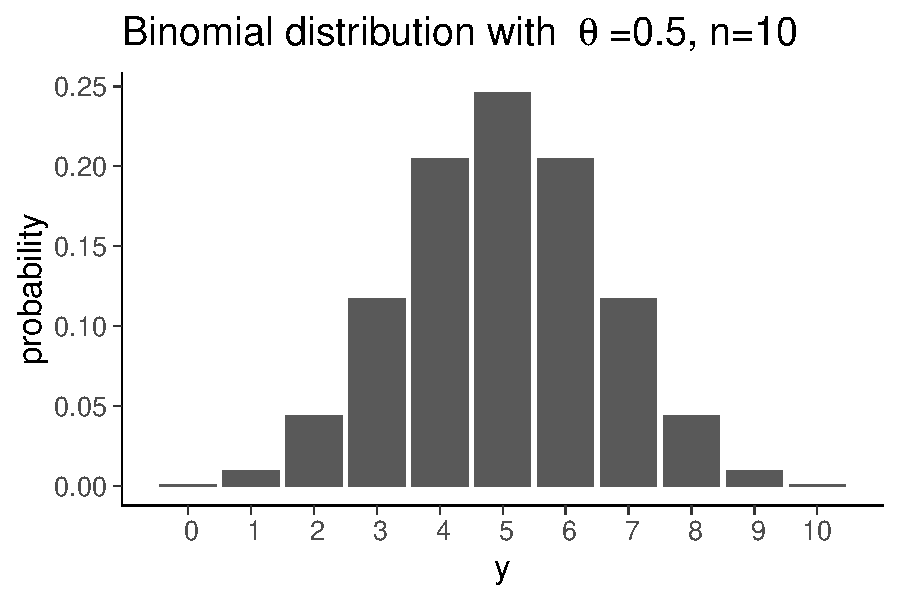
\includegraphics[width=9cm]{dbinom10.pdf}\\
      \vspace{-0.6\baselineskip}
\uncover<2>{\hspace{-18mm}\scriptsize    $p({\color{red}y}|n=10,\theta=0.5)$:\, 0.00 0.01 0.04 0.12 0.21 0.25 0.21 0.12 0.04 0.01 0.00}}
\end{center}
\end{frame}

\begin{frame}
  \frametitle{Binomial: known $\theta$}

  \begin{itemize}
  \item {\color{blue}Observation model} (function of {\color{red} $y$}, discrete)
    \begin{align*}
      p({\color{red}y}|\theta,n) = \binom{n}{{\color{red}y}} \theta^{\color{red}y}(1-\theta)^{n-{\color{red}y}}
    \end{align*}
  \end{itemize}

  \begin{center}
  \only<1>{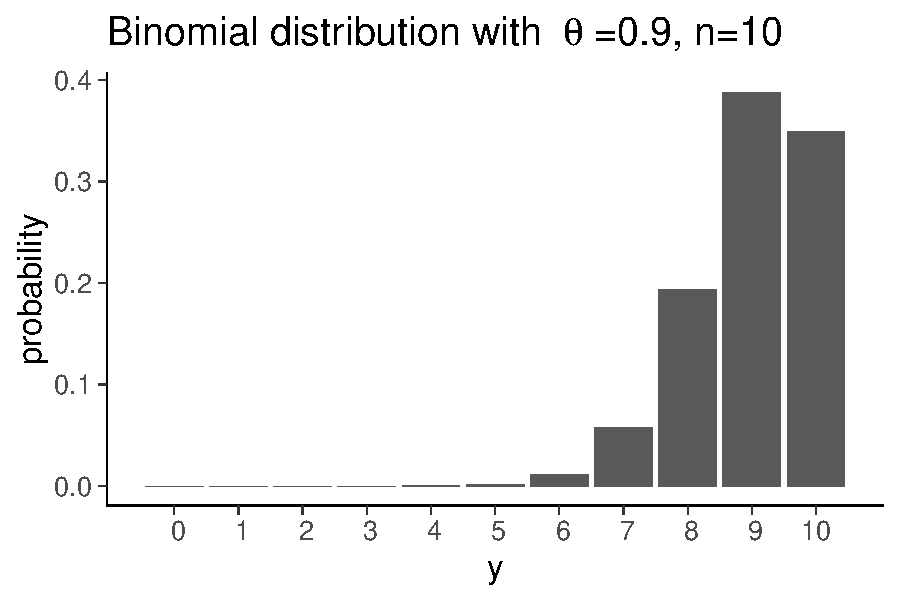
\includegraphics[width=9cm]{dbinom10b.pdf}\\
      \vspace{-0.6\baselineskip}
{\hspace{-18mm}\scriptsize    $p({\color{red}y}|n=10,\theta=0.9)$:\, 0.00 0.00 0.00 0.00 0.00 0.00 0.01 0.06 0.19 0.39 0.35}}
    \only<2>{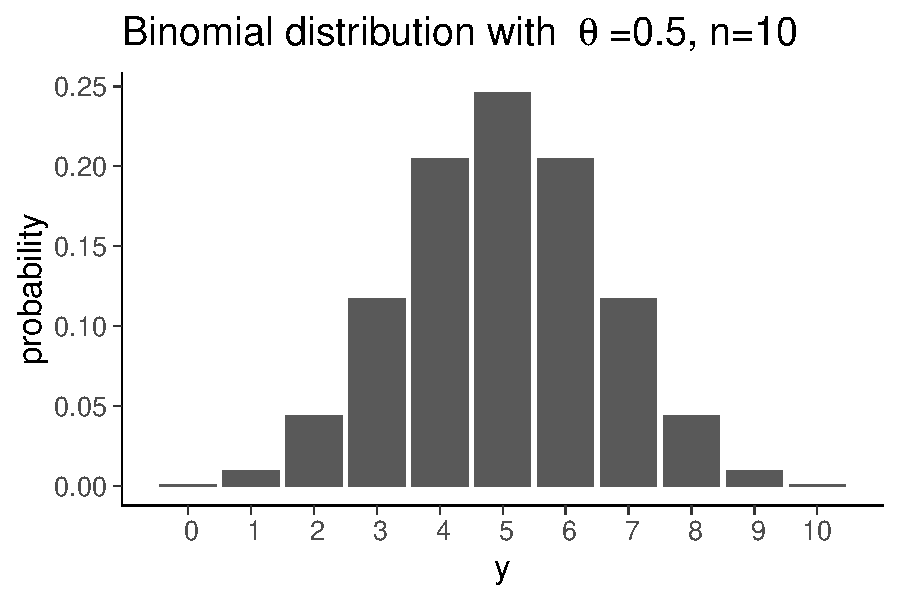
\includegraphics[width=9cm]{dbinom10.pdf}\\
      \vspace{-0.6\baselineskip}
{\hspace{-22mm}\scriptsize    $p({\color{red}y}=6|n=10,\theta=0.5)$:\, 0.00 0.01 0.04 0.12 0.21 0.25 \textbf{0.21} 0.12 0.04 0.01 0.00}}
  \only<3>{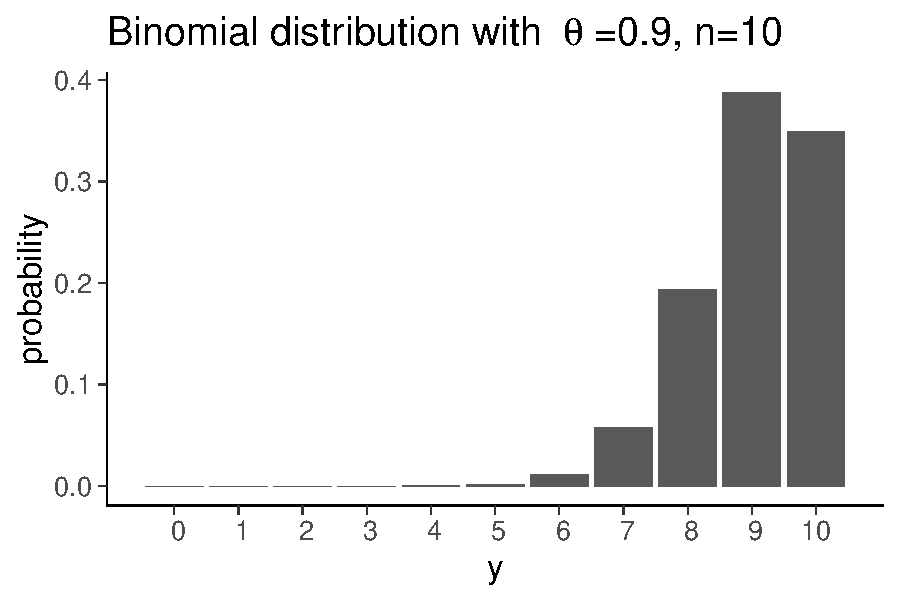
\includegraphics[width=9cm]{dbinom10b.pdf}\\
      \vspace{-0.6\baselineskip}
{\hspace{-22mm}\scriptsize    $p({\color{red}y}=6|n=10,\theta=0.9)$:\, 0.00 0.00 0.00 0.00 0.00 0.00 \textbf{0.01} 0.06 0.19 0.39 0.35}}
\end{center}
\end{frame}

\begin{frame}
  \frametitle{Binomial: unknown $\theta$}

  \begin{itemize}
  \item {\color{blue}Likelihood} (function of {\color{red}$\theta$}, continuous)
    \begin{align*}
      p(y|{\color{red}\theta},n) = \binom{n}{y} {\color{red}\theta}^y(1-{\color{red}\theta})^{n-y}
    \end{align*}
  \end{itemize}

  \begin{center}
    \only<1>{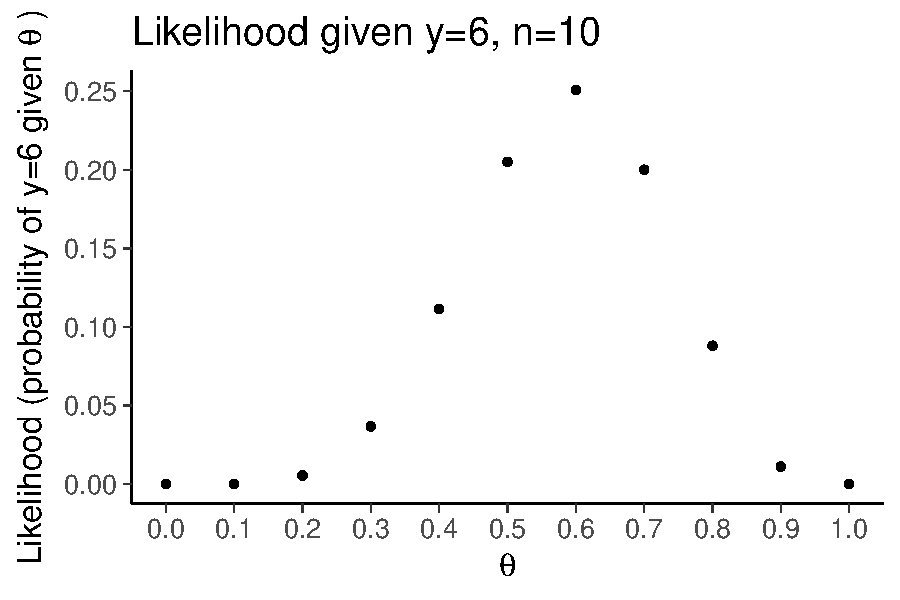
\includegraphics[width=9cm]{lbinom10a.pdf}\\
      \vspace{-0.6\baselineskip}
{\hspace{-12mm}\scriptsize $p(y=6|n=10,{\color{red}\theta})$:\, 0.00\, 0.00\, 0.01\,\, 0.04\, 0.11\, \textbf{0.21}\, 0.25\, 0.20\, 0.09\, \textbf{0.01}\,\, 0.00}}
    \only<2>{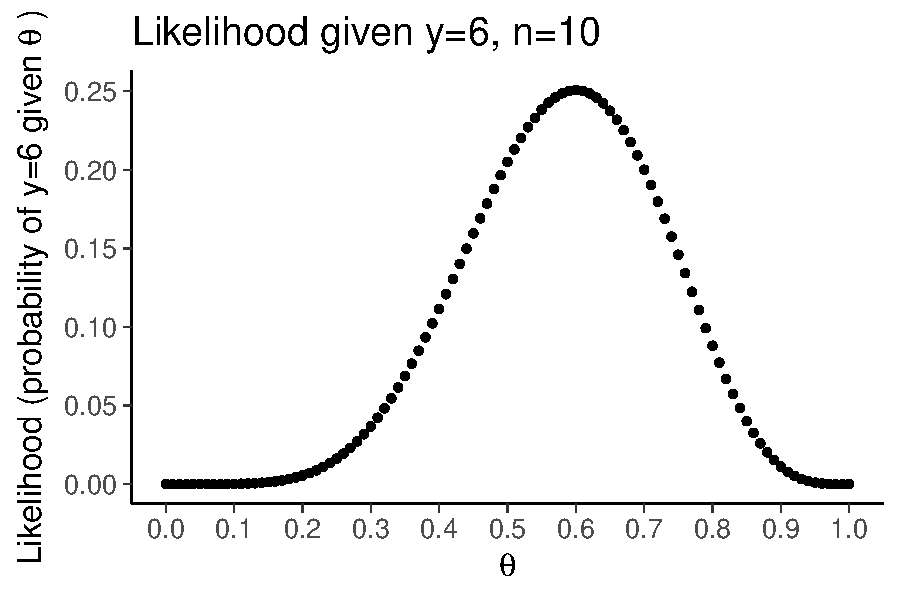
\includegraphics[width=9cm]{lbinom10b.pdf}\\
      \vspace{-0.6\baselineskip}
{\hspace{-14mm}\scriptsize $\,$}}
    \only<3>{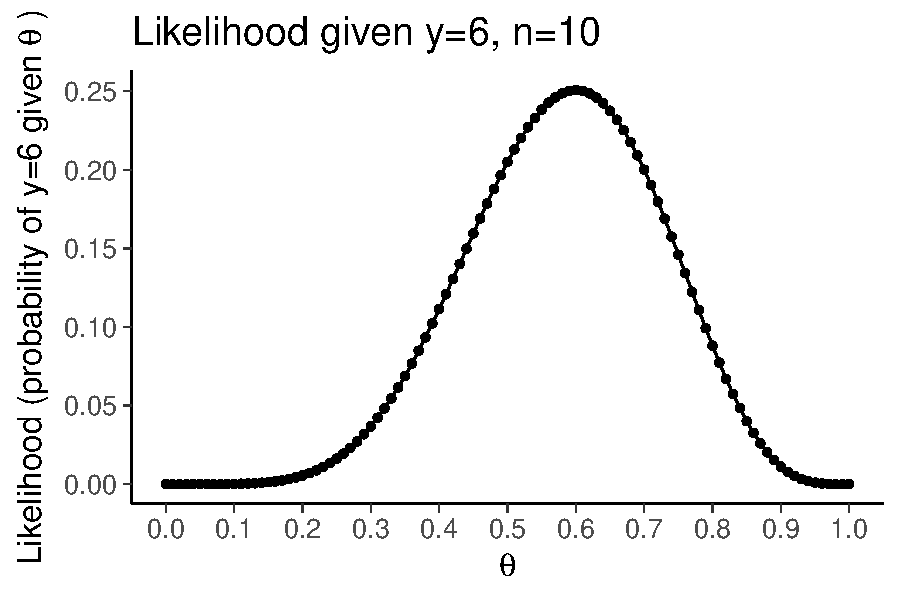
\includegraphics[width=9cm]{lbinom10c.pdf}\\
      \vspace{-0.6\baselineskip}
      \only<3>{\hspace{-14mm}\scriptsize $\,$}}
    \only<4-5>{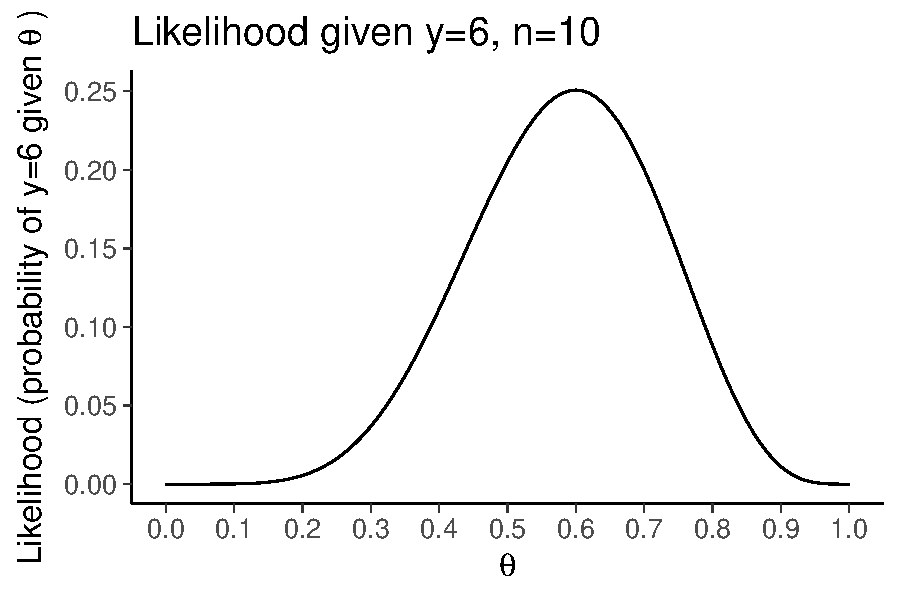
\includegraphics[width=9cm]{lbinom10d.pdf}\\
      \vspace{-0.6\baselineskip}
      \only<4>{\hspace{-14mm}\scriptsize $\,$}
      \only<5>{\scriptsize\texttt{integrate(function({\color{red}theta}) dbinom(6, 10, {\color{red}theta}), 0, 1)} $\approx 0.09$ }}
\end{center}
\end{frame}

\begin{frame}
  \frametitle{Binomial: unknown $\theta$}

  \begin{itemize}
  \item {\color{blue}Posterior} with Bayes rule (function of ${\color{red}\theta}$, continuous)
    \begin{equation*}
      p({\color{red}\theta}|y,n)=\frac{p(y|{\color{red}\theta},n)p({\color{red}\theta}|n)}{p(y|n)}
    \end{equation*}
    \pause
    where $p(y|n)=\int p(y|{\color{red}\theta},n)p({\color{red}\theta}|n) d{\color{red}\theta}$
  \item<3-> Start with uniform prior
    \begin{align*}
      p({\color{red}\theta}|n)=p({\color{red}\theta}|M)=1,\, \text{when}\,\, 0\leq{\color{red}\theta}\leq 1
    \end{align*}
  \item<4-> Then
    \begin{align*}
      p({\color{red}\theta}|y,n)&=\frac{p(y|{\color{red}\theta},n)}{p(y|n)} 
      =\frac{\binom{n}{y} {\color{red}\theta}^y(1-{\color{red}\theta})^{n-y}}{\int_0^1
        \binom{n}{y} {\color{red}\theta}^y(1-{\color{red}\theta})^{n-y} d{\color{red}\theta}} \\
        &=\frac{1}{Z}{\color{red}\theta}^y(1-{\color{red}\theta})^{n-y}
    \end{align*}
  \end{itemize}

\end{frame}

\begin{frame}
  \frametitle{Binomial: unknown $\theta$}

  \begin{itemize}
  \item Normalization term $Z$ (constant given $y$)
    \begin{equation*}
      Z=p(y|n)= \int_0^1 \theta^y(1-\theta)^{n-y} d\theta = \frac{\Gamma(y+1)\Gamma(n-y+1)}{\Gamma(n+2)}
    \end{equation*}
  \item Evaluate with $y=6, n=10$\\
    {\scriptsize\texttt{y<-6;n<-10;\\integrate(function(theta) theta\^{}y*(1-theta)\^{}(n-y), 0, 1)} $\approx 0.0004329$}\\
    \uncover<2->{{\scriptsize\texttt{gamma(6+1)*gamma(10-6+1)/gamma(10+2)} $\approx 0.0004329$}}
  % \item<3-> Normalisation term has \emph{Beta} function form 
  %   \begin{itemize}
  %   \item when integrated over $(0,1)$
  %     the result can presented with Gamma functions
  %   \item with integers  $\Gamma(n)=(n-1)!$
  %   \item for large integers even this is challenging and usually
  %     $\log \Gamma(\cdot)$ is computed instead of $\Gamma(\cdot)$
  %   \end{itemize}
  \end{itemize}

\end{frame}

\begin{frame}
  \frametitle{Binomial: unknown $\theta$}

  \begin{itemize}
  \item Posterior is
    \begin{align*}
      p(\theta|y,n) = \frac{\Gamma(n+2)}{\Gamma(y+1)\Gamma(n-y+1)}\theta^y(1-\theta)^{n-y},
    \end{align*}
    {
    which is called Beta distribution
    \begin{align*}
      \theta|y,n \sim \text{Beta}(y+1,n-y+1)
    \end{align*}}
  \end{itemize}
  \vspace{0.5\baselineskip}
  \begin{center}
    {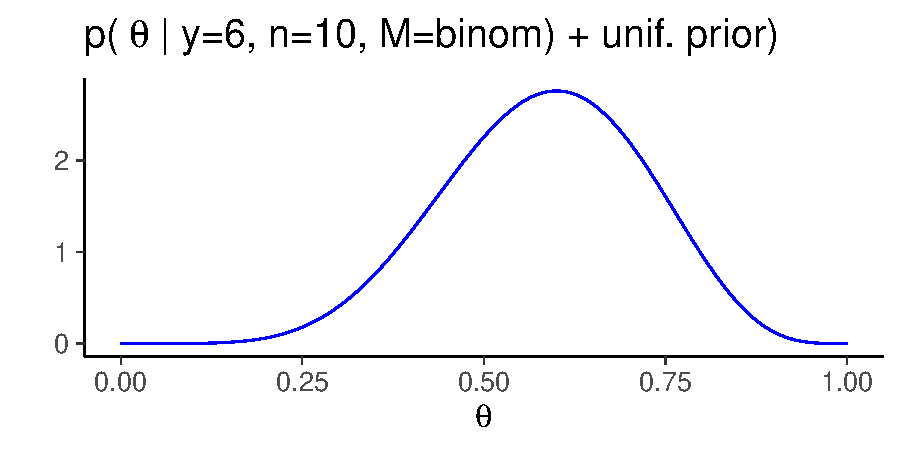
\includegraphics[width=9cm]{dbbeta10c.pdf}}
  \end{center}
\end{frame}

\begin{frame}
  \frametitle{Binomial: unknown $\theta$}

  Sometimes conditioning on the model $M$ is explicitly shown
  
  \begin{itemize}
  \item {\color{blue}Posterior} with Bayes rule (function of $\theta$, continuous)
    \begin{equation*}
      p(\theta|y,n,M)=\frac{p(y|\theta,n,M)p(\theta|n,M)}{p(y|n,M)}
    \end{equation*}
    where $p(y|n,M)=\int p(y|\theta,n,M)p(\theta|n,M) d\theta$
    \vspace{0.5\baselineskip}
    \uncover<2->{\begin{itemize}
    \item makes it more clear that likelihood and prior are both part
      of the model
    \item makes it more clear that there is no absolute probability
      for $p(y|n)$, but it depends on the model $M$
    \item in case of two models, we can evaluate marginal likelihoods
      $p(y|n,M_1)$ and $p(y|n,M_2)$ (more in Ch 7)
    \item<3-> usually dropped to make the notation more concise
    \end{itemize}}
  \end{itemize}

\end{frame}


\end{document}

